\chapter{Design}
\section{Actors}
The main actors of the application are: 
\begin{itemize}
	\item \emph{Non-Logged User (Guest User)} : anonymous users that access the application. They can either sign up or log in.
	\item \emph{Reviewer (User)} : end-user of the application.
	\item \emph{Company Manager} : it's a special kind of \emph{user}, who is granted more benefits. Company Managers identify Game Producers/Publishers that, as such, are able to view and run analytics over their own products. 
	\item \emph{Administrator} : \emph{users} that can run and view analytics that concern the whole database. They are the ones who menage the application: they are able to delete any type of content, update information about Games or Users and to ban them at the occurrence. 
\end{itemize}
\section{Requirements}
\subsection{Functional Requirements}
What follows is a list of the functional requirements.
\subsubsection{Guest User}
\begin{itemize}
	\item sign up
        \item log in
\end{itemize}
\subsubsection{All Users}
\begin{itemize}
	\item view other users' profiles
	\item view companies' profiles
	\item view information about videogames
\end{itemize}
\subsubsection{All Users except Guest Users}
\begin{itemize}
        \item view recommended games
	\item view recommended users
        \item follow/unfollow users
        \item "like" a review
	\item view and edit their profile info
        \item review a videogame
	\item comment on another user's review
	\item delete their reviews
	\item delete their comments
\end{itemize}
\subsubsection{Company Manager Exclusive}
Note: all of the following apply only to games made or produced by the company the \emph{company manager} represents 
\begin{itemize}
	\item add a videogame to the database 
	\item modify info about a game 
	\item delete a videogame from the database 
	\item view the score distribution for the company's videogames
	\item view the top games by average score
	\item view the best game of the company (by average score)
\end{itemize}
\subsubsection{Administrator Exclusive}
\begin{itemize}
	\item delete ("ban") a user from the database
	\item delete a review from the database
	\item delete a comment from the database
	\item delete a videogame from the database 
	\item view the top users by number of likes received on their reviews
	\item view the top users by number of reviews published
	\item view the most active user
	\item view the user with most likes received
	\item view the global distribution of the review score
\end{itemize}
\subsection{Non-Functional Requirements}
The following is a list of all non-functional requirements.
\begin{itemize}
	\item \emph{Usability}: the application must have a user-friendly interface and have low response times
	\item \emph{Availability}: the service provided by the application must be always available to all users
	\item \emph{Reliability}: the application must be stable during its use and it must return reproducible results
	\item \emph{Flexibility}: company managers should be able to add more attributes to a game they want to add, and the application should account for this
	\item \emph{Portability}: the application must be executable in different operating systems without changes in its behaviour
	\item \emph{Privacy}: every user's information should be handled securely
	\item \emph{Maintainability}: the code should be modular and easy to read.
\end{itemize}
\section{Use Case Diagram}
We can look at the use case diagram of the application in Figure \ref{fig:usecase}
\begin{figure}[hbt!]
	\centering
	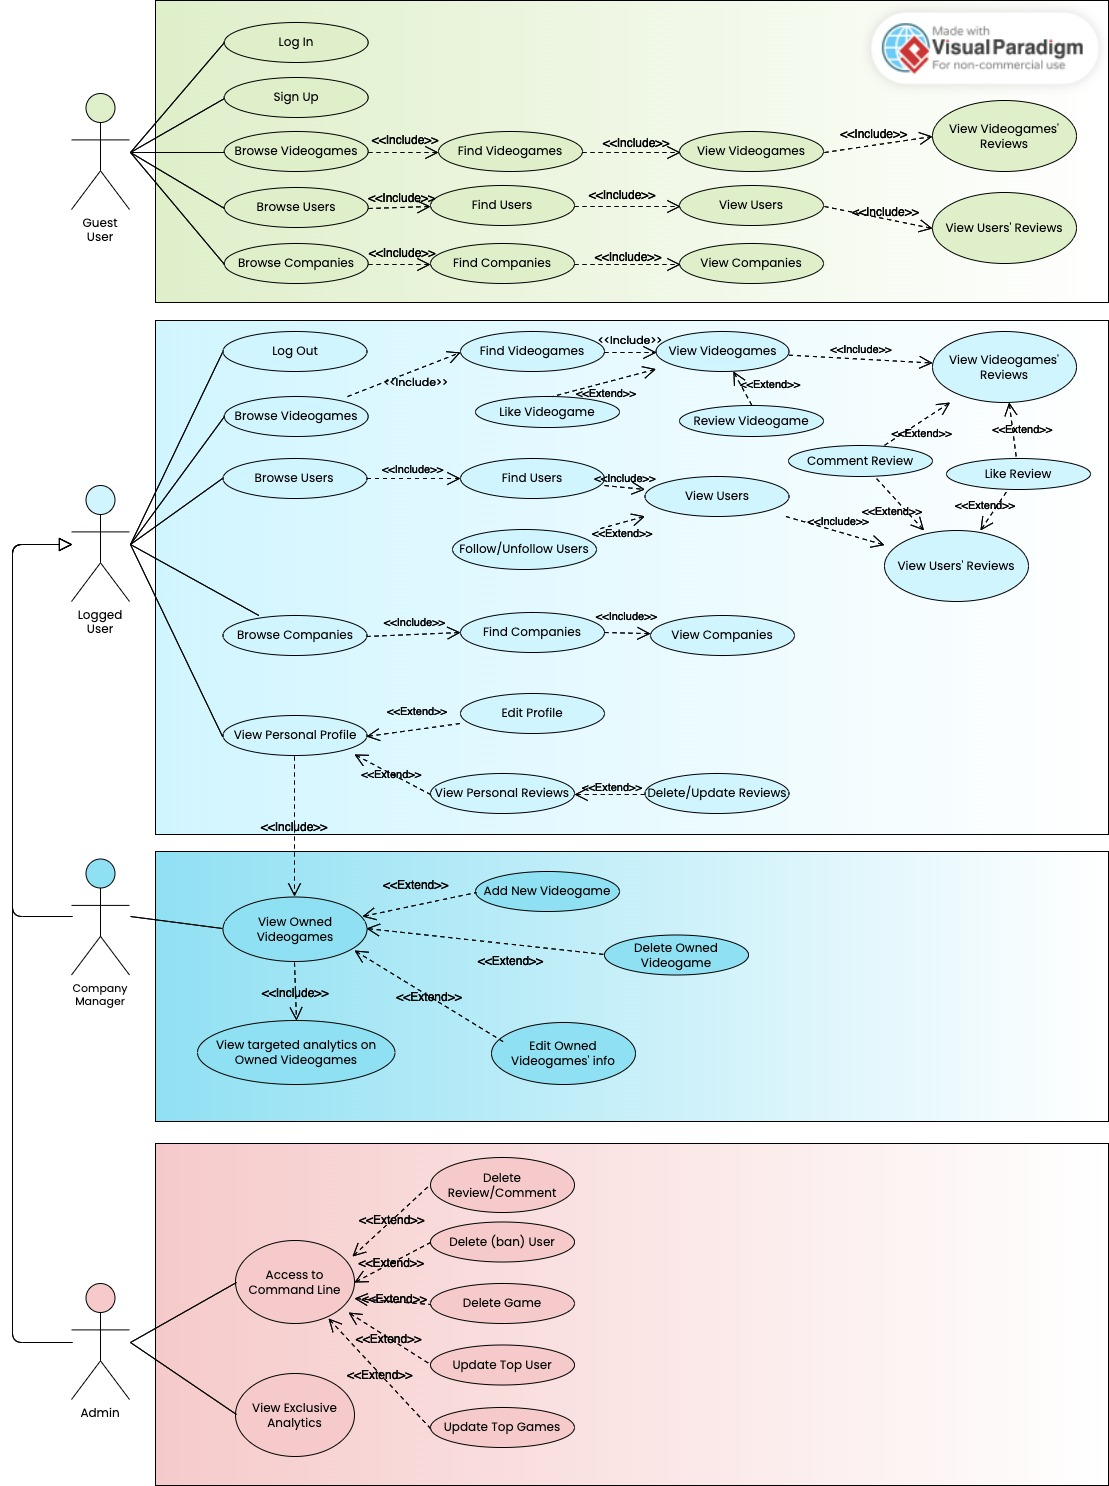
\includegraphics[width=1\textwidth]{chapter3/img/usecase.jpg}
	\caption{Actors and main supported functionalities}
	\label{fig:usecase}
\end{figure}
A \emph{guest user} is able to 
\section{UML Class Diagram}
\begin{figure}[hbt!]
	\centering
	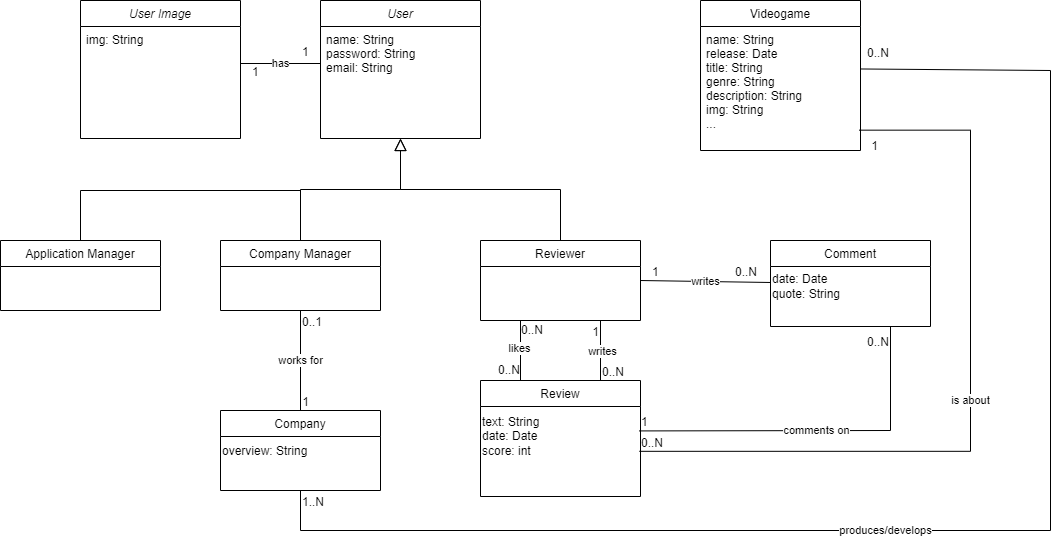
\includegraphics[width=1\textwidth]{chapter3/img/uml.png}
	\caption{UML Class Diagram}
	\label{fig:uml}
\end{figure}
The UML class diagram is reported in Figure \ref{fig:uml}
\subsection{Classes}
A \emph{User} can be either be a \emph{Reviewer}, a \emph{Company Manager} or an \emph{Administrator}. 
\section{Data Models and Implementation}
\subsection{Document DB Collections}
\subsubsection{Videogames}
Whenever a new videogame is inserted, the following attributes are mandatory:
\begin{itemize}
	\item Videogames 
            \begin{itemize}
	       \item Videogames 
            \end{itemize}
	\item Users
	\item Reviews 
	\item Comments 
	\item userImages 
\end{itemize}
\subsection{Document DB Relationships}
\subsection{Document DB Examples}
\begin{python}
    {
	"Name": "(Almost) Total Mayhem",
	"Released": "January 14th, 2011 on Xbox 360",
	"Publishers": "Peanut Gallery",
	"Developers": "Peanut Gallery",
	"Genre": "Action",
	"Perspective": "Side view",
	"Gameplay": "Platform",
	"Setting": "Fantasy",
	"Media Type": "Download",
	"Multiplayer Options": "Same/Split-Screen",
	"Number of Offline Players": "1-2 Players",
	"Description": "description",
	"user_review": 6.0,
	"reviews": [
	{
		"score": 8,
		"quote": "stunning graphhcs!",
		"author": "Yusoreqa",
		"date": "2023-10-30",
		"source": "random",
		"comments": [
		{
			"author": "Hojosu",
			"quote": "I see that Yusoreqa agrees with me.",
			"date": "2023-12-06"
		}
		]
	}
	]
}
\end{python}
\subsection{Graph DB - Neo4j}
\begin{figure}[t]
	\centering
	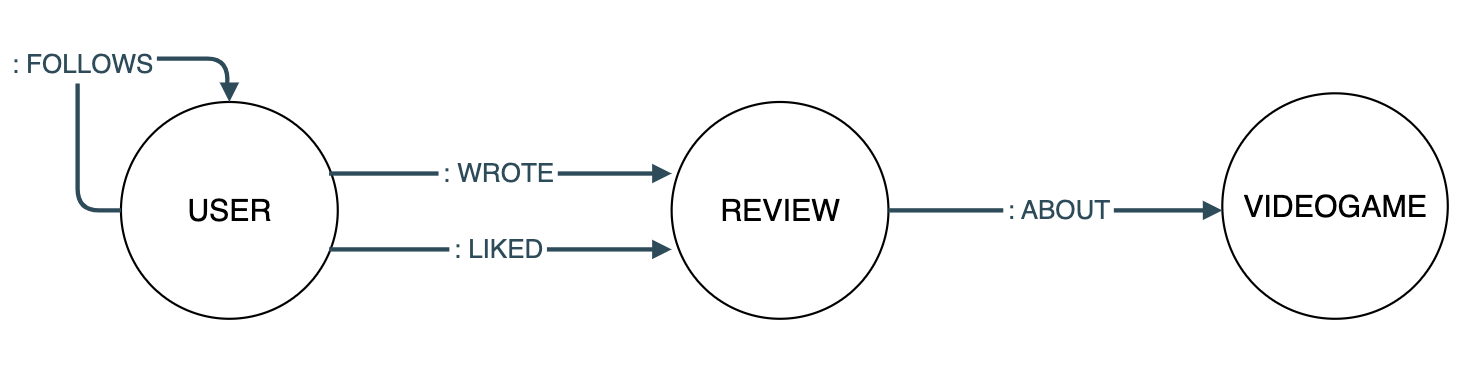
\includegraphics[width=1\textwidth]{chapter3/img/graph.png}
	\caption{Entities handled by \emph{GraphDB} and their relationships}
	\label{fig:graph}
\end{figure}
We handled the following entities via GraphDB (figure \ref{fig:graph}) :
\begin{itemize}
	\item Users 
	\item Videogames 
	\item Reviews
\end{itemize}
\section{Distributed Database Design}
Eventual consistency is sufficient, enforcing strong consistency would be too costly. 
\subsection{Replicas}
\begin{figure}[t]
	\centering
	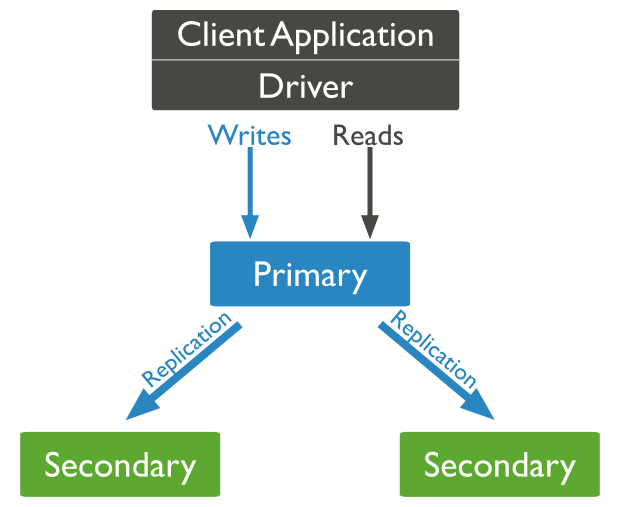
\includegraphics[width=0.5\textwidth]{chapter3/img/replica.png}
	\caption{Replica Set}
	\label{fig:replica}
\end{figure}
We were given the chance to exploit a cluster of three nodes for the project. We deployed one \emph{MongoDB replica} for each node (replicas were not implemented for \emph{Neo4j} since to do so we would have needed the \emph{Enterprise edition}). 
The \emph{primary} is the only member in the replica set that receives write operations (figure \ref{fig:replica}). MongoDB applies write operations on the primary and then records the operations on the primary's \emph{oplog}. \emph{Secondary} members replicate this log and apply the operations to their data sets.
All members of the replica set can accept read operations. By default, however, an application directs its read operations to the primary node.
\subsubsection{Write Concern}
Write concern describes the level of acknowledgment requested from MongoDB for write operations to Replica sets
(TO DO: relation with Async)
\subsection{Sharding}
Heavy loads on a server,  than in the specific case of our application may be due to a large number of users in our network, can be dealt with through a process of horizontal partitioning. Horizontal partitioning of a document database is often referred to as \emph{sharding} and it consists in dividing a database by documents into different sections (known as \emph{shards}) stored on separate servers. This process could be exploited to enable our document database to scale in order to meet a possibly growing demand for our application. Each server within the document database cluster will have only \emph{one} shard per server, so if our database is configured to replicate data, than a single shard will be stored on multiple servers. To implement sharding, we need to select a \emph{shard key} and a \emph{partitioning method}. The shard key specifies the values to use when grouping documents into different shards, so it is represented by one or more fields that need to exist in \emph{all} documents in a collection, and that should be chosen accordingly to the specific requests we expected to get from our clients, in order to optimize the response of the application. 
We can implement sharding for Reviews and Comments, using their \emph{IDs}. 
We shard users and reviews 

%\emph{mongos} instances will pass the \emph{write concern} on to the shards
\subsection{Handling inter-databases consistency}
\begin{figure}[t]
	\centering
	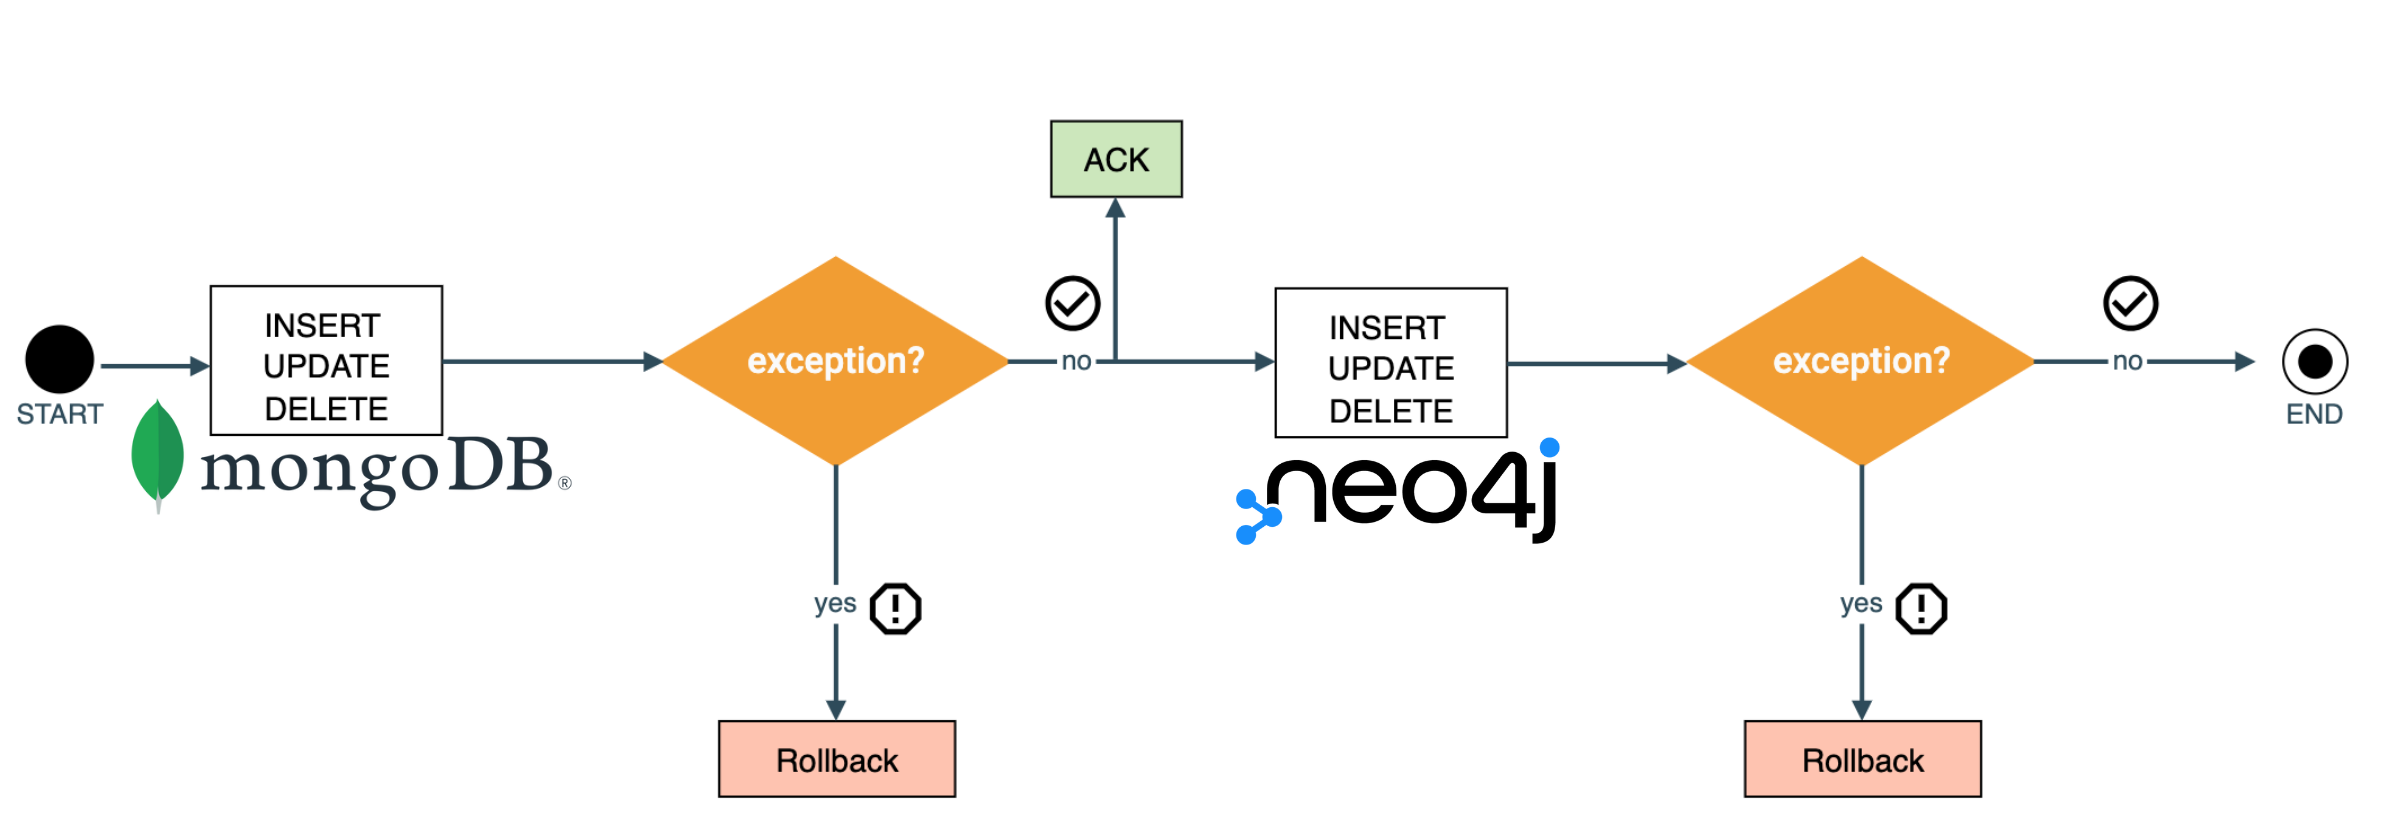
\includegraphics[width=1\textwidth]{chapter3/img/rollback.png}
	\caption{Handling consistency between \emph{MongoDB} and \emph{Neo4j}}
	\label{fig:rb}
\end{figure}
Having to deal with two different architectures (\emph{DocumentDB} and \emph{GraphDB}), we need to face the problem of redundancy and handle the consistency of data that are stored within both databases. 
Any rollback triggered by a failure of an insert, an update or a delete operation, can lead to inconsistencies. 
To address this problem, whenever a write operation  is performed successfully on \emph{MongoDB}, an ACK (\emph{acknowledgement}) is sent to the user. Data on \emph{GraphDB} will be eventually consistent: if any exception occurs when the updates over data on \emph{Neo4j} are attempted, than a rollback operation will be executed in order to bring back both the databases in a consistent state (just as shown in figure \ref{fig:rb}).
% NEW 
Whenever the systems performs an operation that leads to changes (insertions or updates) over the data stored in \emph{Neo4j} we handle possible exceptions, testing for errors in the execution of the code as follows: if an error occurs in the \emph{try} block, we wait for a certain amount of time and we try to re-execute the operations (into the \emph{catch} statement) until it is carried out correctly. 
We do this up to a defined maximum number of times $N = 10$, and at each try the time that the system will wait to make the next attempt will increase. Hopefully, by doing this, even when the server is down the operations will still be carried out once the server will get back up. If $N$ or the chosen time in between every try,  turn out to be not sufficient for the operation to be carried out correctly, than an error will be reported in the \emph{log} file. 
\subsubsection{Eventual Consistency}
Eventual consistency is dealt with by exploiting the \emph{asynchronous execution support} in \emph{Spring} and the \emph{@Async} annotation.
The caller will not have to wait for the complete execution of the called method: annotating a method of a bean with \emph{@Async} will make it execute in a separate thread. 